% Bao cao Nhom 14 theo mau Springer LNCS, ban tieng Viet.
% Bien dich bang XeLaTeX (hoac Tectonic):  xelatex bao_cao.tex
% Mau goc cua Springer giu nguyen o samplepaper.tex de tham khao.
\documentclass[runningheads]{llncs}
%
% Tieng Viet: dung fontspec thay cho [T1]{fontenc} cua mau goc
\usepackage{fontspec}
% Tren Windows dung Times New Roman, tren Linux/Docker dung TeX Gyre Termes (ban Times co du dau tieng Viet)
\IfFontExistsTF{Times New Roman}{\setmainfont{Times New Roman}}{\setmainfont{TeX Gyre Termes}}
\usepackage{amsmath}
\usepackage{graphicx}
\usepackage{booktabs}
\usepackage{array}
\usepackage{color}
\usepackage[hidelinks]{hyperref}
\renewcommand\UrlFont{\color{blue}\rmfamily}
\urlstyle{rm}
%
% Viet hoa cac nhan co dinh cua lop llncs
\renewcommand{\abstractname}{Tóm tắt.}
\renewcommand{\keywordname}{{\bfseries Từ khóa:}}
\renewcommand{\refname}{Tài liệu tham khảo}
\renewcommand{\figurename}{Hình}
\renewcommand{\tablename}{Bảng}
\renewcommand{\ackname}{Lời cảm ơn.}
\renewcommand{\proofname}{Chứng minh}
%
% Hinh lay tu notebook, da cat bo tieu de ve san (xem hinh/README.txt)
\graphicspath{{hinh/}}
%
\begin{document}
%
\title{Kiểm chứng ngưỡng CVSS 8,0 của CSA và đề xuất công thức ưu tiên vá lỗ hổng kết hợp CVSS, EPSS và KEV}
\titlerunning{Kiểm chứng ngưỡng CVSS 8,0 và công thức ưu tiên vá}
%
% TODO: dien ten thanh vien nhom
\author{Nhóm 14}
\authorrunning{Nhóm 14}
\institute{Học phần Chính sách và Quản trị an ninh mạng}
%
\maketitle
%
\begin{abstract}
Báo cáo của Cloud Security Alliance (CSA) ngày 02/04/2026 cho rằng mô hình ngôn ngữ lớn
đã vượt ngưỡng tự động tạo mã khai thác, và khuyến nghị vá trong 48 giờ các lỗ hổng có
CVSS trên 8,0 ảnh hưởng tới hệ thống phơi ra Internet. Chúng tôi kiểm chứng khuyến nghị
này trên 240.409 lỗ hổng có điểm CVSS~3.x (1999--2025), dùng danh mục Known Exploited
Vulnerabilities (KEV) của CISA làm căn cứ về việc bị khai thác thực tế. Ngưỡng 8,0 vừa vá
thừa (98,69\% lỗ hổng trong diện vá khẩn cấp chưa ghi nhận bị khai thác) vừa bỏ sót
(44,14\% lỗ hổng KEV có CVSS dưới 8,0). Chúng tôi đề xuất điểm ưu tiên
$S = AC \times \mathit{CVSS} \times [\mathit{KEV} + (1-\mathit{KEV})\,\mathit{EPSS}^{0{,}3}] \times 10$,
kết hợp mức nghiêm trọng, xác suất bị khai thác theo EPSS, trạng thái KEV và mức quan trọng
của tài sản. Kiểm thử ngược tại ba ngày đánh giá cho thấy khi chỉ vá 1--5\% số lỗ hổng,
công thức bắt được số lỗ hổng sắp bị khai thác nhiều gấp 2,7 đến 8,9 lần so với xếp theo
CVSS. Mức $S \ge 70$ chiếm 1,34\% khối lượng vá nhưng chứa lỗ hổng sắp vào KEV nhiều gấp
khoảng 13 lần ngẫu nhiên, so với 2,3 lần của quy tắc CSA. Tuy vậy, công thức không dự báo
tốt hơn EPSS dùng riêng, 27\% lỗ hổng KEV là zero-day không thể chấm điểm trước, và hệ số
tài sản chưa kiểm chứng được.

\keywords{CVSS \and EPSS \and CISA KEV \and Ưu tiên vá lỗ hổng \and Quản lý lỗ hổng \and Chính sách an ninh mạng.}
\end{abstract}
%
% =====================================================================
\section{Giới thiệu}
% =====================================================================

Mỗi năm có hàng chục nghìn lỗ hổng mới được công bố: riêng năm 2025 có 45.387 lỗ hổng
có điểm CVSS~3.x trong cơ sở dữ liệu NVD. Không tổ chức nào đủ nhân lực và thời gian bảo
trì để vá ngay tất cả, nên câu hỏi thực tế của quản trị an ninh mạng là \emph{vá lỗ hổng
nào trước}. Một chính sách ưu tiên tốt phải tập trung nguồn lực có hạn vào những lỗ hổng
thực sự bị khai thác.

Báo cáo \emph{Automated Exploit Generation: LLMs Cross the Threshold} của
CSA~\cite{csa2026} lập luận rằng mô hình ngôn ngữ lớn (LLM) đã rút ngắn khoảng thời gian
từ khi công bố lỗ hổng đến khi có mã khai thác, và đưa ra một khuyến nghị chính sách cụ
thể: coi các CVE có CVSS trên 8,0 ảnh hưởng tới hệ thống phơi ra Internet là trường hợp
khẩn cấp, mục tiêu khắc phục trong 48 giờ. Khuyến nghị này đơn giản và dễ áp dụng, nhưng
dựa hoàn toàn vào điểm CVSS, vốn đo \emph{mức nghiêm trọng} chứ không đo \emph{khả năng
bị khai thác}.

Báo cáo này trả lời ba câu hỏi:
\begin{enumerate}
\item[\textbf{CH1.}] Trên dữ liệu thực, quy tắc ngưỡng CVSS 8,0 vá thừa và bỏ sót bao nhiêu lỗ hổng bị khai thác?
\item[\textbf{CH2.}] Một công thức kết hợp CVSS, EPSS, KEV và mức quan trọng của tài sản có sắp thứ tự ưu tiên tốt hơn không, khi chỉ dùng thông tin có tại thời điểm ra quyết định?
\item[\textbf{CH3.}] Công thức đó có khả thi để triển khai trong thực tế không, và giới hạn của nó ở đâu?
\end{enumerate}

\noindent Đóng góp của báo cáo gồm: (i) phân tích bài báo gốc và tách khuyến nghị
chính sách có thể kiểm chứng được; (ii) đánh giá định lượng ngưỡng 8,0 trên 240.409 lỗ
hổng; (iii) đề xuất công thức điểm ưu tiên $S$; (iv) kiểm chứng $S$ bằng kiểm thử ngược
có chống rò rỉ dữ liệu tương lai, kèm đánh giá tính khả thi và các hạn chế được nêu rõ.

Phần~\ref{sec:baibao} phân tích bài báo gốc. Phần~\ref{sec:lienquan} tóm tắt các nghiên
cứu liên quan. Phần~\ref{sec:nentang} trình bày kiến thức nền tảng. Phần~\ref{sec:giaiphap}
mô tả giải pháp đề xuất. Phần~\ref{sec:trienkhai} mô tả phương án triển khai và cách đánh
giá. Phần~\ref{sec:ketqua} báo cáo kết quả thực nghiệm. Phần~\ref{sec:khathi} đánh giá tính
khả thi. Phần~\ref{sec:ketluan} kết luận.

% =====================================================================
\section{Phân tích bài báo gốc}\label{sec:baibao}
% =====================================================================

\subsection{Vấn đề bài báo giải quyết}

Bài báo của CSA~\cite{csa2026} là một báo cáo tổng hợp (whitepaper, 20 trang) thuộc
chương trình AI Safety Initiative. Câu hỏi trung tâm là: LLM đã thực sự làm thay đổi cán
cân tấn công -- phòng thủ chưa, cụ thể là đã đủ khả năng đi từ \emph{phát hiện lỗ hổng}
tới \emph{vũ khí hóa} (tạo mã khai thác hoạt động được) chưa. Kết luận của CSA là ngưỡng
này đã bị vượt qua: chi phí và kỹ năng cần để biến một mô tả CVE thành mã khai thác đã
giảm mạnh.

\subsection{Bằng chứng bài báo sử dụng}

Bài báo không có thực nghiệm riêng mà tổng hợp các kết quả đã công bố:
\begin{itemize}
\item \textbf{Nghiên cứu của UIUC}~\cite{fang2024}: GPT-4 khai thác thành công 87\% trong 15
lỗ hổng one-day khi được cung cấp mô tả CVE, nhưng chỉ 7\% khi không có mô tả.
\item \textbf{PwnGPT} (ACL 2025): khung tự động tạo mã khai thác nhị phân, nâng tỷ lệ
hoàn thành bài CTF từ 26,3\% lên 57,9\% với o1-preview.
\item \textbf{DARPA AIxCC} (2025): các hệ thống tự động phát hiện 86\% lỗ hổng tổng hợp và
tìm ra 18 lỗ hổng thật chưa từng biết.
\item \textbf{Google Big Sleep} và \textbf{CVE-2025-37899}: LLM tìm ra lỗ hổng thật trong
SQLite và trong mô-đun ksmbd của nhân Linux.
\item \textbf{Incalmo} (2025): tấn công nhiều bước thành công 37/40 môi trường mạng mô phỏng,
mất 12--54 phút, chi phí dưới 15 USD.
\item \textbf{Sử dụng thực tế}: nhóm tấn công cấp nhà nước dùng LLM từ 2024; vụ việc tại
Mexico (2025--2026) được báo chí mô tả là dùng LLM tạo mã khai thác.
\end{itemize}

\subsection{Khuyến nghị chính sách được kiểm chứng}

Trong mục \emph{Organizational Vulnerability Management in the New Environment}, bài báo
viết: \emph{``Security teams should treat published CVEs affecting internet-exposed systems
with CVSS scores above 8.0 as requiring emergency patching timelines \ldots\ CSA recommends
organizations target remediation within 48 hours for such vulnerabilities''}. Phần kết luận
nhắc lại yêu cầu rà soát thời gian vá cho lỗ hổng ``CVSS 8.0+'' trên hệ thống phơi ra Internet.

Đây là khuyến nghị duy nhất trong bài có dạng một \emph{quy tắc định lượng}, nên kiểm
chứng được bằng dữ liệu. Chúng tôi diễn đạt nó thành quy tắc:
\begin{equation}
\text{vá khẩn cấp} \iff \mathit{CVSS} \ge 8{,}0 \;\wedge\; \text{hệ thống phơi ra Internet}.
\label{eq:csa}
\end{equation}

\subsection{Nhận xét về bài báo}

Có bốn điểm đáng chú ý khi đánh giá khuyến nghị này:
\begin{enumerate}
\item Bài báo ghi rõ là \emph{``Unofficial AI-assisted Research''}, chưa qua quy trình
xét duyệt chính thức của CSA.
\item Lập luận ``LLM rút ngắn thời gian tạo mã khai thác'' dẫn tới kết luận ``phải vá
nhanh hơn'', nhưng không trả lời \emph{lỗ hổng nào} sẽ bị nhắm tới. Ngưỡng 8,0 không được
bài báo giải thích hay kiểm chứng.
\item Chính bài báo cũng viết \emph{``Prioritization frameworks should weight exploitability
heavily''}, tức nên coi trọng khả năng bị khai thác. Điều này mâu thuẫn một phần với việc
chọn CVSS, vốn là thước đo mức nghiêm trọng, làm tiêu chí duy nhất.
\item Điều kiện ``hệ thống phơi ra Internet'' phụ thuộc vào tài sản của từng tổ chức, không
có trong dữ liệu công khai. Vì vậy phần kiểm chứng của chúng tôi áp ngưỡng 8,0 cho mọi lỗ
hổng, và đưa yếu tố tài sản vào công thức đề xuất dưới dạng hệ số $AC$.
\end{enumerate}

% =====================================================================
\section{Các nghiên cứu liên quan}\label{sec:lienquan}
% =====================================================================

\paragraph{CVSS và giới hạn của nó.}
Allodi và Massacci~\cite{allodi2014} dùng phương pháp nghiên cứu ca -- chứng (case-control)
và chỉ ra rằng vá theo điểm CVSS cao gần như tương đương vá ngẫu nhiên xét về giảm rủi ro
bị khai thác; yếu tố có giá trị hơn là việc đã tồn tại mã khai thác. Bản đặc tả CVSS
v3.1~\cite{cvss31} cũng nêu rõ điểm cơ sở (Base Score) đo mức nghiêm trọng, không phải rủi ro.

\paragraph{Dự đoán khả năng bị khai thác.}
Jacobs và cộng sự~\cite{jacobs2020} so sánh các chiến lược vá và cho thấy mô hình dự đoán
khai thác đạt hiệu quả cao hơn nhiều so với quy tắc ngưỡng CVSS ở cùng khối lượng vá. Nhóm
này sau đó phát triển EPSS~\cite{jacobs2021}, mô hình học máy công khai cho xác suất một
CVE bị khai thác trong 30 ngày tới, hiện do FIRST duy trì và cập nhật hằng ngày~\cite{epss}.

\paragraph{Danh mục lỗ hổng đã bị khai thác.}
CISA ban hành Chỉ thị BOD 22-01~\cite{bod2201} năm 2021, yêu cầu các cơ quan liên bang Mỹ
vá lỗ hổng trong danh mục KEV~\cite{kev} theo hạn định. KEV trở thành nguồn công khai phổ
biến nhất về việc lỗ hổng bị khai thác thực tế.

\paragraph{Khung ra quyết định nhiều yếu tố.}
SSVC~\cite{ssvc} của CERT/CC đề xuất cây quyết định dựa trên tình trạng khai thác, mức
độ phơi nhiễm và tác động tới nhiệm vụ, thay cho một điểm số đơn lẻ. Shimizu và
Hashimoto~\cite{shimizu2026} đề xuất cây quyết định VMC xét lần lượt KEV, EPSS rồi CVSS để
xếp lỗ hổng vào bốn nhóm ưu tiên. Công thức của chúng tôi gần với VMC về thứ tự xét các
yếu tố, nhưng cho ra điểm liên tục 0--100 và có thêm hệ số tài sản.

% =====================================================================
\section{Kiến thức nền tảng}\label{sec:nentang}
% =====================================================================

\subsection{CVE và NVD}
CVE (Common Vulnerabilities and Exposures) là mã định danh chuẩn của một lỗ hổng, ví dụ
\texttt{CVE-2021-44228}. NVD~\cite{nvd} của NIST là cơ sở dữ liệu công khai lưu mô tả và
điểm CVSS của mọi CVE. Mỗi CVE có thể có hai điểm: điểm do NVD chấm (\emph{Primary}) và điểm
do đơn vị công bố chấm (CNA). Lỗ hổng bị hủy có trạng thái \emph{Rejected}.

\subsection{CVSS}
CVSS v3.x~\cite{cvss31} tính điểm cơ sở 0--10 từ hai nhóm chỉ số: \emph{khả năng khai thác
kỹ thuật} (đường tấn công AV, độ phức tạp AC, quyền cần có PR, tương tác người dùng UI) và
\emph{tác động} (tính bí mật C, toàn vẹn I, sẵn sàng A, phạm vi S). Ví dụ vector
\[\texttt{AV:N/AC:L/PR:N/UI:N/S:U/C:H/I:H/A:H}\]
cho điểm 9,8. Điểm CVSS mô tả \emph{nếu bị khai
thác thì hậu quả nặng đến đâu}, nhưng không cho biết kẻ tấn công \emph{có} nhắm tới lỗ hổng
đó hay không.

\subsection{EPSS}
EPSS~\cite{jacobs2021,epss} là mô hình học máy ước lượng xác suất một CVE bị khai thác trong
30 ngày tới, dựa trên đặc trưng của lỗ hổng (nhà cung cấp, loại lỗi, mã khai thác công khai,
nhắc đến trên mạng xã hội\ldots) và dữ liệu khai thác quan sát được. Điểm nằm trong $[0, 1]$,
cập nhật hằng ngày, có lưu lịch sử theo ngày. Phân bố EPSS rất lệch: 64\% lỗ hổng trong
dữ liệu của chúng tôi có EPSS từ 0,001 đến dưới 0,01. Mô hình EPSS có nhiều phiên bản; trong
giai đoạn nghiên cứu xuất hiện các phiên bản v2022.01.01, v2023.03.01 và v2025.03.14.

\subsection{CISA KEV}
KEV~\cite{kev} là danh mục lỗ hổng đã được CISA xác nhận bị khai thác thực tế, mỗi mục ghi
ngày được đưa vào (\texttt{dateAdded}). Chúng tôi dùng KEV làm \emph{căn cứ đúng} (ground
truth) cho việc bị khai thác. KEV là căn cứ thận trọng: lỗ hổng không có trong KEV chưa chắc
không bị khai thác, chỉ là chưa được CISA xác nhận.

\subsection{Mức quan trọng của tài sản}
Trong quản lý lỗ hổng, cùng một lỗ hổng gây rủi ro khác nhau tùy tài sản chứa nó. Nhóm chỉ
số môi trường (Environmental) của CVSS và yếu tố \emph{Mission Impact} của SSVC đều phản ánh
điều này. Mức quan trọng của tài sản thường lấy từ cơ sở dữ liệu quản lý cấu hình (CMDB) hoặc
danh mục tài sản của tổ chức, và không có dữ liệu công khai.

\subsection{Đánh giá một quy tắc ưu tiên}
Một quy tắc ưu tiên chia lỗ hổng thành nhóm ``vá'' và ``chưa vá''. Đối chiếu với KEV cho
ma trận nhầm lẫn với bốn ô: vá đúng (TP), vá thừa (FP), bỏ sót (FN), bỏ qua đúng (TN). Từ
đó có \emph{độ chính xác} (precision) $= TP/(TP+FP)$, tức tỷ lệ lỗ hổng bị khai thác trong
nhóm phải vá, và \emph{độ bao phủ} (recall) $= TP/(TP+FN)$, tức tỷ lệ lỗ hổng bị khai thác
được ưu tiên. Khi so sánh các cách xếp hạng, cần cố định \emph{cùng khối lượng vá}, vì quy
tắc vá nhiều hơn luôn bắt được nhiều hơn.

\subsection{Kiểm thử ngược và rò rỉ dữ liệu tương lai}
Kiểm thử ngược (backtesting) đánh giá một phương pháp bằng cách đứng ở một ngày $T$ trong
quá khứ, chỉ dùng thông tin có tại $T$, rồi đối chiếu với những gì xảy ra sau $T$. Lỗi
thường gặp là \emph{rò rỉ dữ liệu tương lai} (data leakage): điểm EPSS hiện tại của một lỗ
hổng đã bị khai thác thường rất cao \emph{vì} việc khai thác đã xảy ra, nên dùng EPSS hiện
tại để ``dự đoán'' quá khứ sẽ cho kết quả đẹp giả tạo. Vì vậy mọi phép kiểm chứng phải dùng
EPSS lịch sử đúng ngày $T$.

% =====================================================================
\section{Giải pháp đề xuất}\label{sec:giaiphap}
% =====================================================================

\subsection{Công thức điểm ưu tiên}

Chúng tôi đề xuất điểm ưu tiên $S$ cho mỗi cặp (lỗ hổng, tài sản):
\begin{equation}
S = AC \times \mathit{CVSS} \times \left[\mathit{KEV} + (1-\mathit{KEV}) \times \mathit{EPSS}^{0{,}3}\right] \times 10,
\label{eq:S}
\end{equation}
trong đó $AC \in [0,1]$ là mức quan trọng của tài sản, $\mathit{CVSS} \in [0,10]$,
$\mathit{KEV} \in \{0,1\}$ bằng 1 nếu lỗ hổng đã có trong KEV tại thời điểm đánh giá,
$\mathit{EPSS} \in [0,1]$ là điểm EPSS tại thời điểm đánh giá. Do đó $S \in [0, 100]$; lỗ
hổng có $S$ càng cao càng phải vá sớm.

\subsection{Ý nghĩa từng thành phần}

Vì $\mathit{KEV}$ chỉ nhận 0 hoặc 1, biểu thức trong ngoặc vuông thực chất là một phép rẽ
nhánh:
\begin{equation}
S =
\begin{cases}
AC \times \mathit{CVSS} \times 10 & \text{nếu đã có trong KEV,}\\[2pt]
AC \times \mathit{CVSS} \times \mathit{EPSS}^{0{,}3} \times 10 & \text{nếu chưa có trong KEV.}
\end{cases}
\label{eq:S2}
\end{equation}

\begin{itemize}
\item \textbf{Nhánh KEV.} Lỗ hổng đã bị khai thác thì không cần dự đoán nữa: hệ số khả năng
bị khai thác bằng 1, thứ tự chỉ còn phụ thuộc mức nghiêm trọng và tài sản.
\item \textbf{Nhánh chưa KEV.} Mức nghiêm trọng được điều chỉnh theo xác suất bị khai thác.
Đây là phần mang tính dự đoán và là phần cần chứng minh.
\item \textbf{Số mũ 0,3.} Phần lớn lỗ hổng có EPSS rất nhỏ. Nhân thẳng EPSS sẽ làm điểm dồn
về 0 và CVSS mất tác dụng. Số mũ 0,3 nén thang EPSS mà vẫn giữ thứ tự:
$0{,}001 \mapsto 0{,}13$, $0{,}01 \mapsto 0{,}25$, $0{,}1 \mapsto 0{,}50$, $0{,}9 \mapsto 0{,}97$.
\item \textbf{Hệ số $AC$.} Cùng một lỗ hổng, nằm trên máy chủ thanh toán ($AC=1$) phải vá
trước khi nằm trên máy thử nghiệm ($AC=0{,}2$). Hệ số này cũng là chỗ đưa điều kiện ``phơi ra
Internet'' của CSA vào công thức.
\end{itemize}

\subsection{Ví dụ}

Bảng~\ref{tab:vidu} so sánh thứ tự theo $S$ (với $AC=1$) và theo quy tắc CSA trên bốn lỗ
hổng giả định. Quy tắc CSA chọn A và D, bỏ qua B (90\% khả năng bị khai thác) và C (đã bị
khai thác). Công thức $S$ xếp B và C lên đầu.

\begin{table}
\centering
\caption{Ví dụ tính điểm $S$ với $AC = 1$ (số liệu giả định).}\label{tab:vidu}
\begin{tabular}{cccccc}
\toprule
Lỗ hổng & CVSS & EPSS & KEV & $S$ & Quy tắc CSA \\
\midrule
A & 9,8 & 0,001 & 0 & $9{,}8 \times 0{,}13 \times 10 \approx 12$ & vá khẩn cấp \\
B & 7,5 & 0,90  & 0 & $7{,}5 \times 0{,}97 \times 10 \approx 73$ & bỏ qua \\
C & 6,5 & --    & 1 & $6{,}5 \times 1 \times 10 = 65$           & bỏ qua \\
D & 9,0 & 0,10  & 0 & $9{,}0 \times 0{,}50 \times 10 \approx 45$ & vá khẩn cấp \\
\bottomrule
\end{tabular}
\end{table}

\subsection{Phạm vi chứng minh}

Nhánh KEV không cần chứng minh vì lỗ hổng đã bị khai thác. Phần cần chứng minh là nhánh
chưa KEV: điểm $\mathit{CVSS} \times \mathit{EPSS}^{0{,}3}$ có xếp những lỗ hổng \emph{sắp}
bị khai thác lên trên không. Do không có dữ liệu tài sản công khai, mọi thực nghiệm đặt
$AC = 1$. Hệ số 10 chỉ đổi thang điểm, không đổi thứ tự.

% =====================================================================
\section{Phương án triển khai và cách đánh giá}\label{sec:trienkhai}
% =====================================================================

\subsection{Dữ liệu}

Toàn bộ dữ liệu là công khai và miễn phí (Bảng~\ref{tab:dulieu}). Mã nguồn chỉ đọc siêu dữ
liệu mô tả lỗ hổng: không tạo mã khai thác, không quét hay tấn công hệ thống nào.

\begin{table}
\centering
\caption{Nguồn dữ liệu.}\label{tab:dulieu}
\begin{tabular}{p{2.2cm}p{4.6cm}p{4.4cm}}
\toprule
Nguồn & Cách lấy & Dùng để \\
\midrule
NVD (NIST) & Tệp JSON 2.0 theo năm, 2002--2025 (khoảng 300~MB) & Điểm CVSS, ngày công bố \\
CISA KEV & Kho \texttt{cisagov/kev-data}, phiên bản 2026.10.08 & Căn cứ bị khai thác, ngày vào KEV \\
FIRST EPSS & Tệp điểm hằng ngày và API \texttt{api.first.org} & Điểm EPSS lịch sử theo ngày \\
\bottomrule
\end{tabular}
\end{table}

\paragraph{Làm sạch.} Loại lỗ hổng bị hủy; với mỗi lỗ hổng lấy điểm CVSS~3.x, ưu tiên điểm
do NVD chấm, nếu không có thì dùng điểm của CNA. Trong 316.367 lỗ hổng (1999--2025),
240.409 lỗ hổng (75,99\%) có CVSS~3.x và được dùng cho thống kê; 1.570 trong số đó nằm trong
KEV. Lỗ hổng chỉ có CVSS~2.0 được ghi nhận riêng.

\subsection{Quy trình xử lý}

Hệ thống được hiện thực bằng Python (pandas, numpy, matplotlib) dưới dạng bốn notebook
Jupyter chạy được trên Google Colab, cùng một bộ bảy script chạy tuần tự:
\[
\text{Thu thập} \rightarrow \text{làm sạch, ghép theo mã CVE} \rightarrow \text{tính } S
\rightarrow \text{kiểm thử ngược} \rightarrow \text{bảng, hình}.
\]
Hàm tính điểm cốt lõi chỉ gồm một dòng:
\begin{verbatim}
def diem_S(cvss, epss, kev, ac=1.0):
    return ac * cvss * (kev + (1 - kev) * epss ** 0.3) * 10
\end{verbatim}

\subsection{Thực nghiệm 1: đánh giá ngưỡng CVSS 8,0}

Chia 240.409 lỗ hổng theo hai câu hỏi: CVSS có từ 8,0 không, và có trong KEV không, được
ma trận nhầm lẫn. Tính độ chính xác, độ bao phủ, số lỗ hổng phải vá cho mỗi lỗ hổng bị khai
thác bắt được. Lặp lại cho giai đoạn gần đây 2023--2025 và cho các ngưỡng 7,0 và 9,0. Đây là
thực nghiệm \emph{mô tả}: nó dùng trạng thái KEV hiện tại, không phải bài toán dự đoán.

\subsection{Thực nghiệm 2: kiểm thử ngược công thức S}

Chọn ba ngày đánh giá $T \in \{31/12/2023,\ 31/12/2024,\ 30/06/2025\}$. Tại mỗi $T$:
\begin{enumerate}
\item Lấy mọi lỗ hổng đã công bố trước $T$ và có CVSS~3.x.
\item Tách phần đã có trong KEV tại $T$ (nhánh KEV, không cần chứng minh).
\item Với phần chưa có trong KEV, lấy EPSS \emph{của đúng ngày $T$} để chống rò rỉ dữ liệu
tương lai; lỗ hổng không có điểm EPSS coi bằng 0.
\item Tính $S$; gắn nhãn $y = 1$ nếu lỗ hổng vào KEV trong 365 ngày sau $T$.
\item Chia $S$ thành mười mức 10 điểm, đếm tỷ lệ $y=1$ trong mỗi mức.
\item So sánh $S$ với quy tắc CSA, và với xếp theo CVSS, theo EPSS \emph{ở cùng khối lượng
vá} (1\%, 5\%, và bằng số lượng của quy tắc CSA).
\end{enumerate}
Khi nhiều lỗ hổng bằng điểm tại ranh giới chọn (rất phổ biến với CVSS), lấy giá trị kỳ vọng
của việc chọn ngẫu nhiên trong nhóm bằng điểm, nên kết quả có thể là số lẻ. Khoảng tin cậy
95\% của chênh lệch giữa các phương pháp tính bằng bootstrap.

\subsection{Thực nghiệm 3: điểm trước khi vào KEV}

Lấy 836 lỗ hổng vào KEV từ 01/04/2023. Với mỗi lỗ hổng, tính $S$ bằng EPSS của 1 ngày và 30
ngày \emph{trước} ngày vào KEV (nhánh chưa KEV), rồi so với $S$ khi đã vào KEV
($\mathit{CVSS} \times 10$). Thực nghiệm này trả lời: công thức có cảnh báo sớm được không.

\subsection{Thực nghiệm 4: kiểm định giả thuyết đặt trước}

Bộ script \texttt{src/05\_kiem\_chung.py} dùng thiết kế chặt hơn, với giả thuyết cố định
trước khi chạy. Lỗ hổng công bố năm 2023--2025 được chia thành đợt theo tháng; ngày quyết
định là cuối tháng công bố; nhãn là vào KEV trong 180 ngày sau. Năm 2024 và 2025 là năm
kiểm thử; số mũ được chọn lại trên các năm trước (walk-forward). Hai giả thuyết:
\begin{itemize}
\item \textbf{H1.} Ở cùng khối lượng vá với quy tắc CSA, công thức (số mũ 0,3) bắt được
nhiều lỗ hổng bị khai thác hơn CVSS. Đạt nếu khoảng tin cậy 95\% bootstrap (1.000 lần) của
chênh lệch, gộp 2024 và 2025, nằm hoàn toàn trên 0.
\item \textbf{H2.} Trong mô phỏng vá hằng tháng với cùng ngân sách (25\% số lỗ hổng trong
năm), công thức đầy đủ (có KEV) đạt tỷ lệ ``an toàn trong 30 ngày'' cao nhất. Một lỗ hổng
an toàn nếu được vá trước khi bị khai thác hoặc chậm nhất 30 ngày sau.
\end{itemize}
Đối chứng gồm CVSS, EPSS, công thức bỏ thành phần KEV, và nhánh ``High'' của cây quyết định
VMC~\cite{shimizu2026} (EPSS $\ge 0{,}088$ và CVSS $\ge 7{,}0$).

% =====================================================================
\section{Kết quả thực nghiệm}\label{sec:ketqua}
% =====================================================================

\subsection{Ngưỡng CVSS 8,0 vừa vá thừa vừa bỏ sót}

Bảng~\ref{tab:bonnhom} là ma trận nhầm lẫn của quy tắc CSA. Trong 66.722 lỗ hổng phải vá
khẩn cấp, chỉ 877 (1,31\%) nằm trong KEV: trung bình phải vá 76,1 lỗ hổng mới trúng một lỗ
hổng bị khai thác. Ngược lại, 693 trong 1.570 lỗ hổng KEV (44,14\%) có CVSS dưới 8,0 và bị
quy tắc bỏ qua. Giai đoạn 2023--2025 cho kết quả gần như giống hệt: bỏ sót 43,05\%, phải vá
99,3 lỗ hổng cho mỗi lỗ hổng bắt được (Hình~\ref{fig:hailoi}).

\begin{table}
\centering
\caption{Ma trận nhầm lẫn của quy tắc CVSS $\ge 8{,}0$, giai đoạn 1999--2025.}\label{tab:bonnhom}
\begin{tabular}{lrrr}
\toprule
 & Trong KEV & Không trong KEV & Cộng \\
\midrule
CVSS $\ge 8{,}0$ (phải vá) & 877 & 65.845 & 66.722 \\
CVSS $< 8{,}0$ (bỏ qua)   & 693 & 172.994 & 173.687 \\
\midrule
Cộng & 1.570 & 238.839 & 240.409 \\
\midrule
\multicolumn{4}{l}{Độ chính xác $= 877/66.722 = 1{,}31\%$; độ bao phủ $= 877/1.570 = 55{,}86\%$} \\
\bottomrule
\end{tabular}
\end{table}

\begin{figure}
\centering
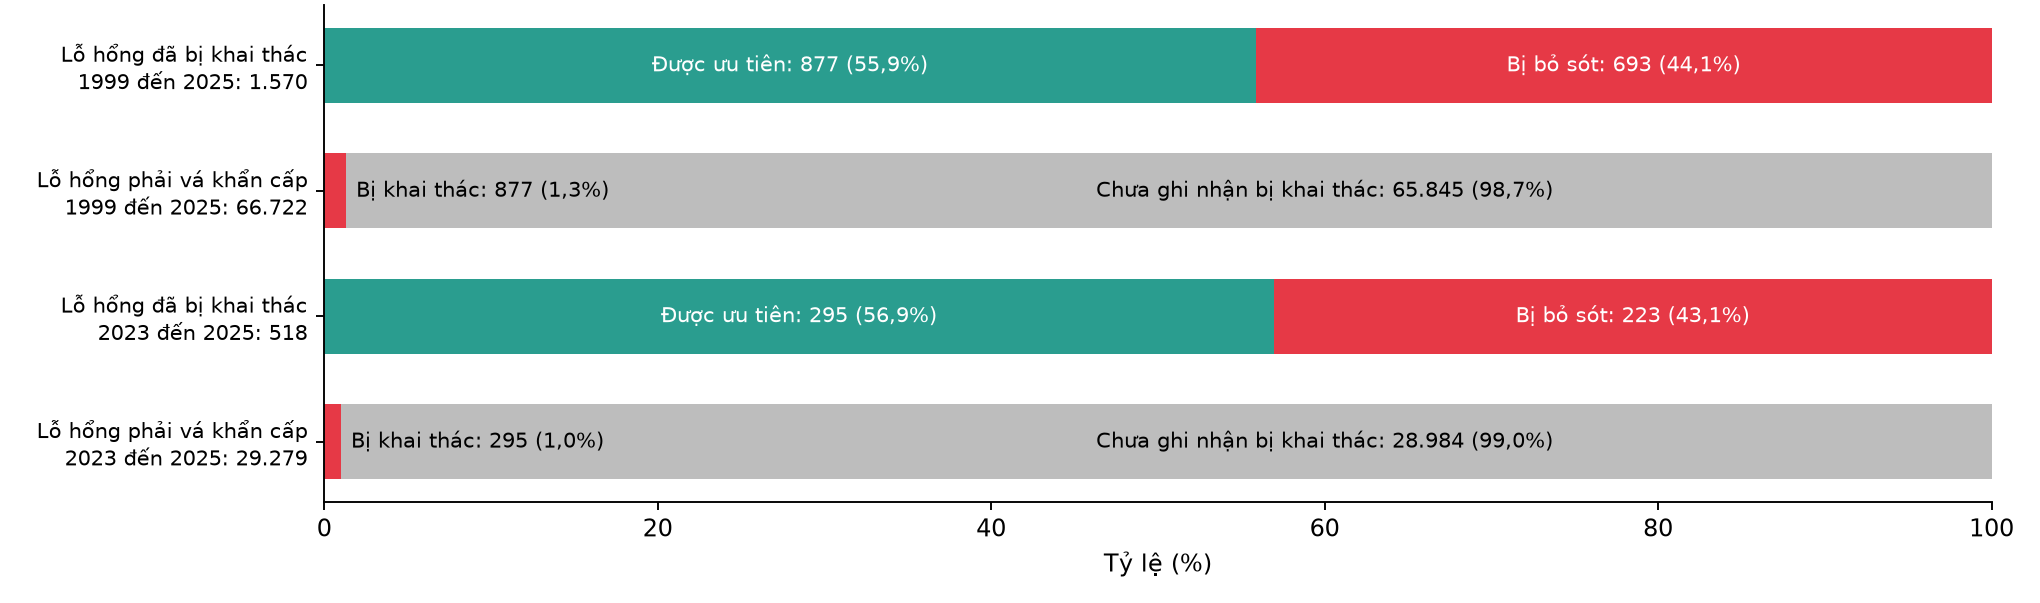
\includegraphics[width=\textwidth]{nguong_hai_loi.png}
\caption{Ngưỡng CVSS 8,0 bỏ sót khoảng 44\% lỗ hổng bị khai thác, trong khi khoảng 99\% lỗ
hổng phải vá khẩn cấp chưa ghi nhận bị khai thác.}\label{fig:hailoi}
\end{figure}

\paragraph{Đổi ngưỡng không giải quyết được vấn đề.} Bảng~\ref{tab:nguong} cho thấy hạ
ngưỡng xuống 7,0 giảm bỏ sót còn 11,40\% nhưng phải vá 54,33\% tổng số lỗ hổng; nâng lên 9,0
thì bỏ sót 65,99\%. Ở mọi ngưỡng, tỷ lệ bị khai thác trong nhóm phải vá chỉ khoảng 1--1,5\%.
Nguyên nhân là CVSS phân biệt kém: xác suất một lỗ hổng nằm trong KEV chỉ tăng từ 0,17\%
(CVSS 4,0--6,9) lên 1,54\% (CVSS 9,0--10).

\begin{table}
\centering
\caption{So sánh các ngưỡng CVSS, giai đoạn 1999--2025.}\label{tab:nguong}
\begin{tabular}{lccc}
\toprule
Ngưỡng & \quad Phải vá\quad & \quad Bỏ sót KEV\quad & Bị khai thác trong nhóm phải vá \\
\midrule
CVSS $\ge 7{,}0$ & 54,33\% & 11,40\% & 1,06\% \\
CVSS $\ge 8{,}0$ (CSA) & 27,75\% & 44,14\% & 1,31\% \\
CVSS $\ge 9{,}0$ & 14,43\% & 65,99\% & 1,54\% \\
\bottomrule
\end{tabular}
\end{table}

\paragraph{Ổn định theo thời gian và nhà cung cấp.} Tỷ lệ lỗ hổng KEV có CVSS dưới 8,0 dao
động 32--57\% qua các năm 2010--2025, không có xu hướng giảm. Trong 693 lỗ hổng bị bỏ sót,
Microsoft chiếm 35,8\%, Apple 7,8\%, Cisco 5,9\%: đây là những sản phẩm phổ biến nhất trong
doanh nghiệp.

\subsection{Điểm S phân biệt được lỗ hổng sắp bị khai thác}

Tại ngày đánh giá 30/06/2025 có 209.623 lỗ hổng chưa có trong KEV, trong đó chỉ 91 (0,043\%)
vào KEV trong 12 tháng sau. Bảng~\ref{tab:mucS} cho thấy tỷ lệ vào KEV tăng theo mức điểm:
các mức từ 70 trở lên có tỷ lệ 1,16--1,29\%, gấp 27--30 lần trung bình. Hình~\ref{fig:mucS}
cho thấy xu hướng này lặp lại ở cả ba ngày đánh giá.

\begin{table}
\centering
\setlength{\tabcolsep}{9pt}
\caption{Phân bố điểm $S$ và tỷ lệ vào KEV trong 12 tháng sau, ngày đánh giá 30/06/2025.}\label{tab:mucS}
\begin{tabular}{lrrrr}
\toprule
Mức $S$ & Số lỗ hổng & Vào KEV & Tỷ lệ & Gấp trung bình \\
\midrule
0 -- dưới 10   & 100.819 & 11 & 0,011\% & 0,3 \\
10 -- dưới 20  & 72.627  & 20 & 0,028\% & 0,6 \\
20 -- dưới 30  & 17.999  & 3  & 0,017\% & 0,4 \\
30 -- dưới 40  & 7.541   & 7  & 0,093\% & 2,1 \\
40 -- dưới 50  & 3.769   & 4  & 0,11\%  & 2,4 \\
50 -- dưới 60  & 2.348   & 5  & 0,21\%  & 4,9 \\
60 -- dưới 70  & 1.717   & 7  & 0,41\%  & 9,4 \\
70 -- dưới 80  & 1.206   & 14 & 1,16\%  & 26,7 \\
80 -- dưới 90  & 777     & 10 & 1,29\%  & 29,6 \\
90 -- 100      & 820     & 10 & 1,22\%  & 28,1 \\
\midrule
Tổng & 209.623 & 91 & 0,043\% & 1,0 \\
\bottomrule
\end{tabular}
\end{table}

\begin{figure}
\centering
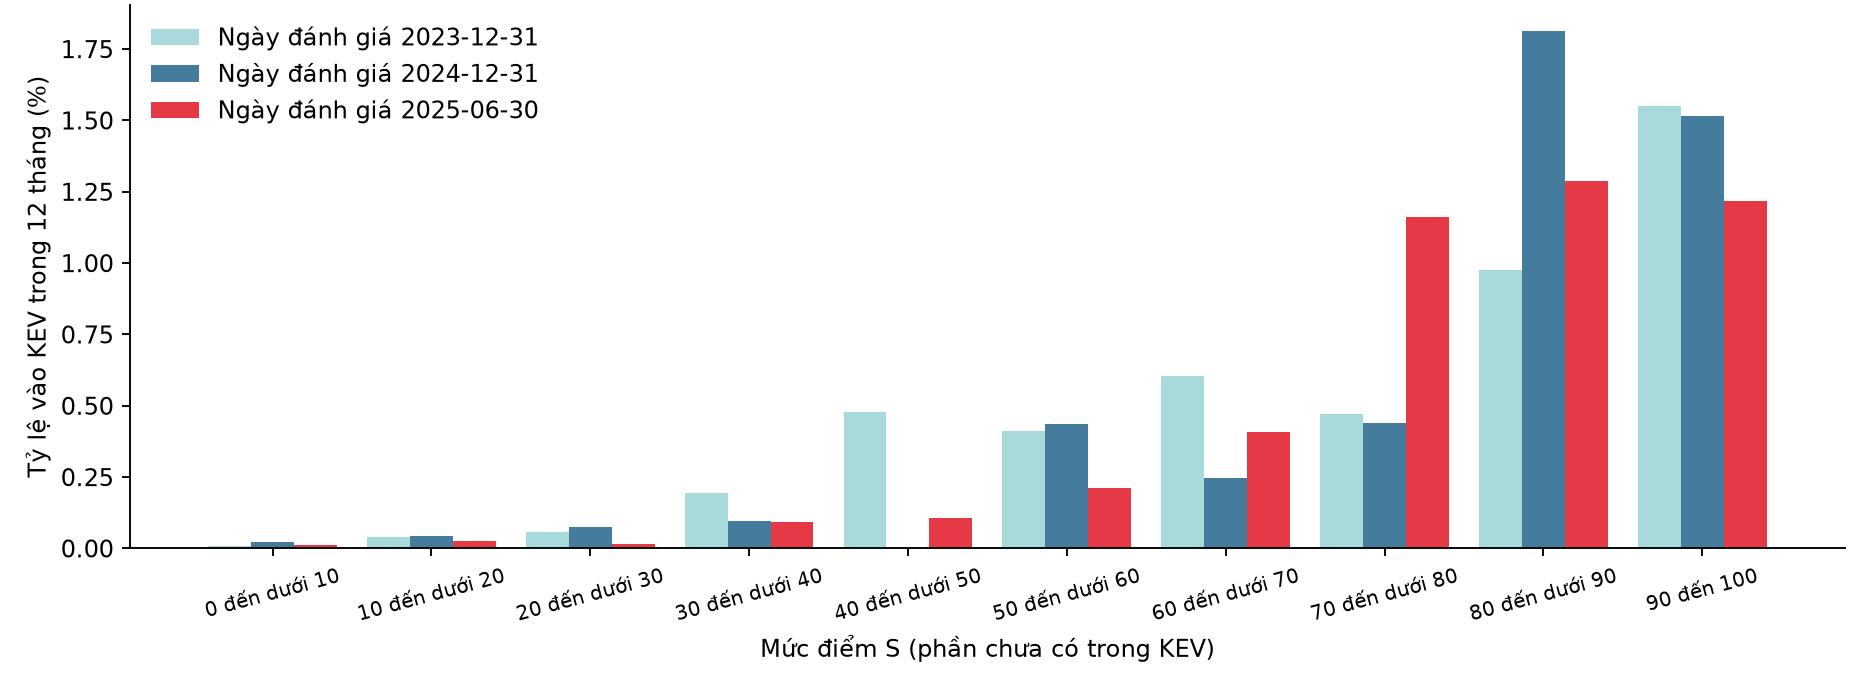
\includegraphics[width=\textwidth]{S_ty_le_theo_muc.png}
\caption{Tỷ lệ vào KEV trong 12 tháng sau theo mức điểm $S$, tại ba ngày đánh giá.}\label{fig:mucS}
\end{figure}

\paragraph{So với quy tắc CSA.} Vá mọi lỗ hổng có $S \ge 70$ nghĩa là vá 2.803 lỗ hổng
(1,34\%) và bắt được 34/91 (37,36\%), tức 82 lỗ hổng phải vá cho mỗi lỗ hổng bắt được. Quy
tắc CSA vá 58.133 lỗ hổng (27,73\%), bắt 54/91 (59,34\%), tức 1.076 lỗ hổng phải vá cho mỗi
lỗ hổng bắt được. Quy tắc CSA bắt được nhiều hơn vì vá nhiều gấp khoảng 20 lần, nhưng hiệu
suất kém khoảng 13 lần.

\paragraph{Cùng khối lượng vá.} Bảng~\ref{tab:cungkl} cố định số lỗ hổng được vá. Khi vá
1\% hoặc 5\%, công thức $S$ bắt được nhiều gấp 2,7 đến 8,9 lần so với xếp theo CVSS, ổn
định ở cả ba ngày; khoảng tin cậy 95\% của chênh lệch đều nằm trên 0. Tuy nhiên $S$ chỉ
tương đương EPSS: bằng nhau ở 2023 và 2024, kém nhẹ ở 2025 (25 so với 30 khi vá 1\%). Hình~\ref{fig:batduoc}
cho thấy đường của $S$ và EPSS gần như trùng nhau ở phần vá ít, và cùng nằm xa phía trên
đường của CVSS.

\begin{table}
\centering
\caption{Số lỗ hổng vào KEV trong 12 tháng bắt được khi vá cùng số lượng.}\label{tab:cungkl}
\begin{tabular}{llrccc}
\toprule
Ngày & Khối lượng & Số vá & CVSS & EPSS & $S$ \\
\midrule
31/12/2023 & 1\%      & 1.473  & 2,0/61  & 14/61 & 14/61 \\
           & 5\%      & 7.365  & 8,9/61  & 30/61 & 30/61 \\
           & như CSA  & 42.685 & 38/61   & 49/61 & 51/61 \\
31/12/2024 & 1\%      & 1.867  & 2,0/80  & 18/80 & 18/80 \\
           & 5\%      & 9.337  & 9,7/80  & 28/80 & 26/80 \\
           & như CSA  & 52.662 & 48/80   & 45/80 & 48/80 \\
30/06/2025 & 1\%      & 2.096  & 4,8/91  & 30/91 & 25/91 \\
           & 5\%      & 10.481 & 11,3/91 & 51/91 & 50/91 \\
           & như CSA  & 58.133 & 54/91   & 65/91 & 65/91 \\
\bottomrule
\end{tabular}
\end{table}

\begin{figure}
\centering
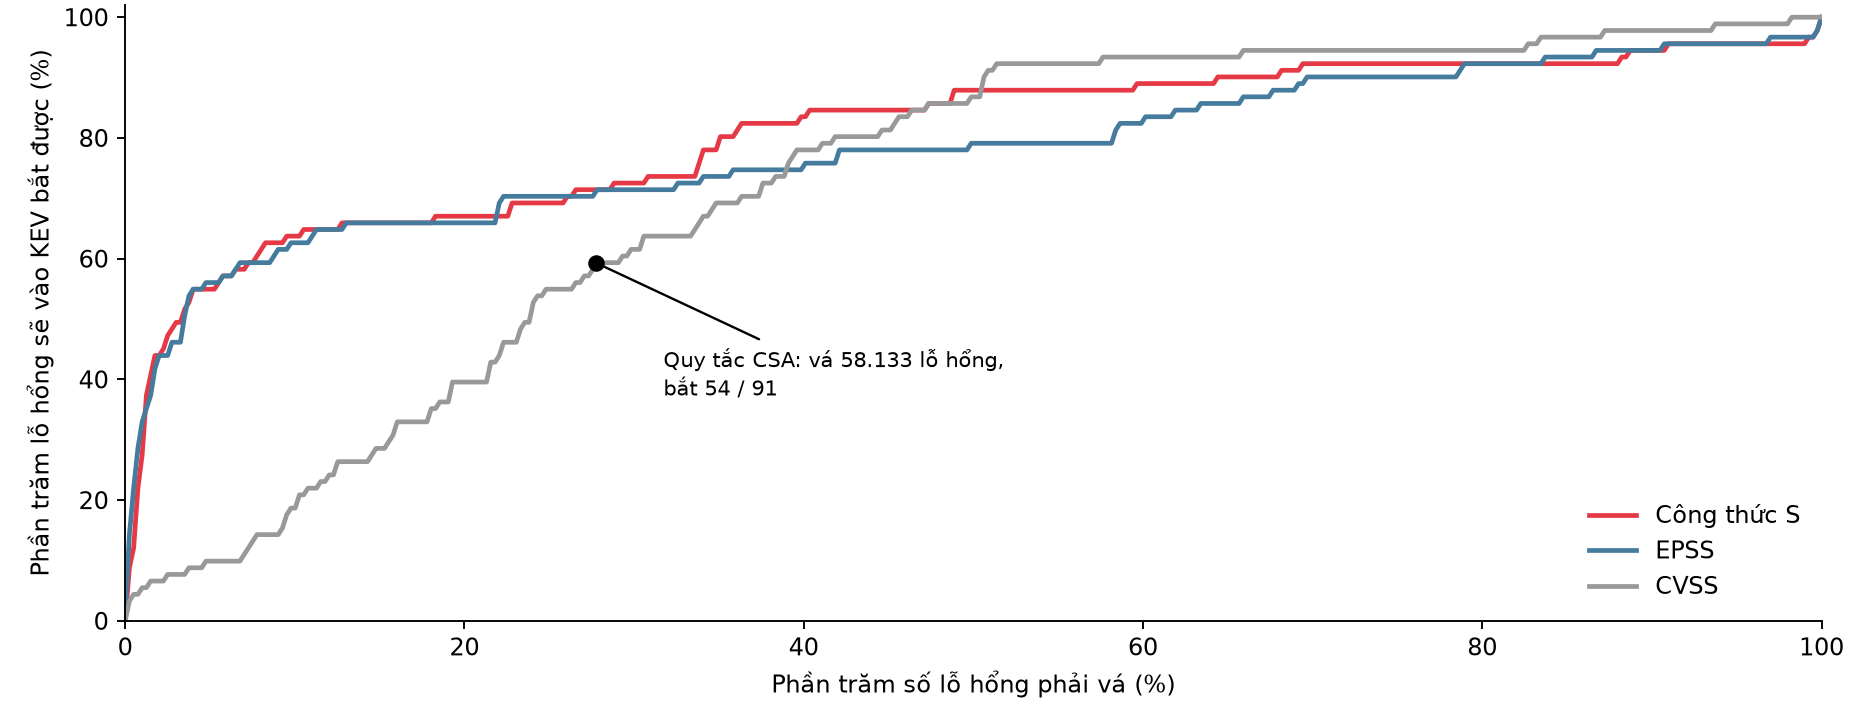
\includegraphics[width=\textwidth]{S_duong_bat_duoc.png}
\caption{Đường bắt được tại ngày 30/06/2025: phần trăm lỗ hổng sẽ vào KEV bắt được theo
phần trăm lỗ hổng phải vá. Chấm đen là quy tắc CSA.}\label{fig:batduoc}
\end{figure}

\subsection{Điểm trước khi vào KEV}

Trong 836 lỗ hổng vào KEV từ 01/04/2023, có 227 lỗ hổng (27,15\%) chưa có điểm EPSS một ngày
trước khi vào KEV; 226 trong số đó được công bố cùng ngày hoặc một ngày trước khi vào KEV.
Đây là các lỗ hổng zero-day: không công thức nào chấm được điểm trước, chỉ nhánh KEV đưa
chúng lên đầu ngay khi được xác nhận.

Với 609 lỗ hổng còn lại, điểm $S$ một ngày trước khi vào KEV thấp hơn nhiều điểm khi vào
KEV (Hình~\ref{fig:truockev}): trung vị khoảng cách là 63 điểm, trung vị tỷ số là 0,19.
Nguyên nhân là EPSS chủ yếu tăng \emph{sau} khi việc khai thác đã được biết đến. Dù vậy, xét
theo hiệu suất (Bảng~\ref{tab:truockev}), mức $S \ge 70$ một ngày trước khi vào KEV chiếm
1,34\% khối lượng vá nhưng chứa 17,73\% lỗ hổng sắp vào KEV, gấp khoảng 13 lần chọn ngẫu
nhiên; quy tắc CSA chứa 64,20\% với 27,73\% khối lượng, chỉ gấp khoảng 2,3 lần.

\begin{figure}
\centering
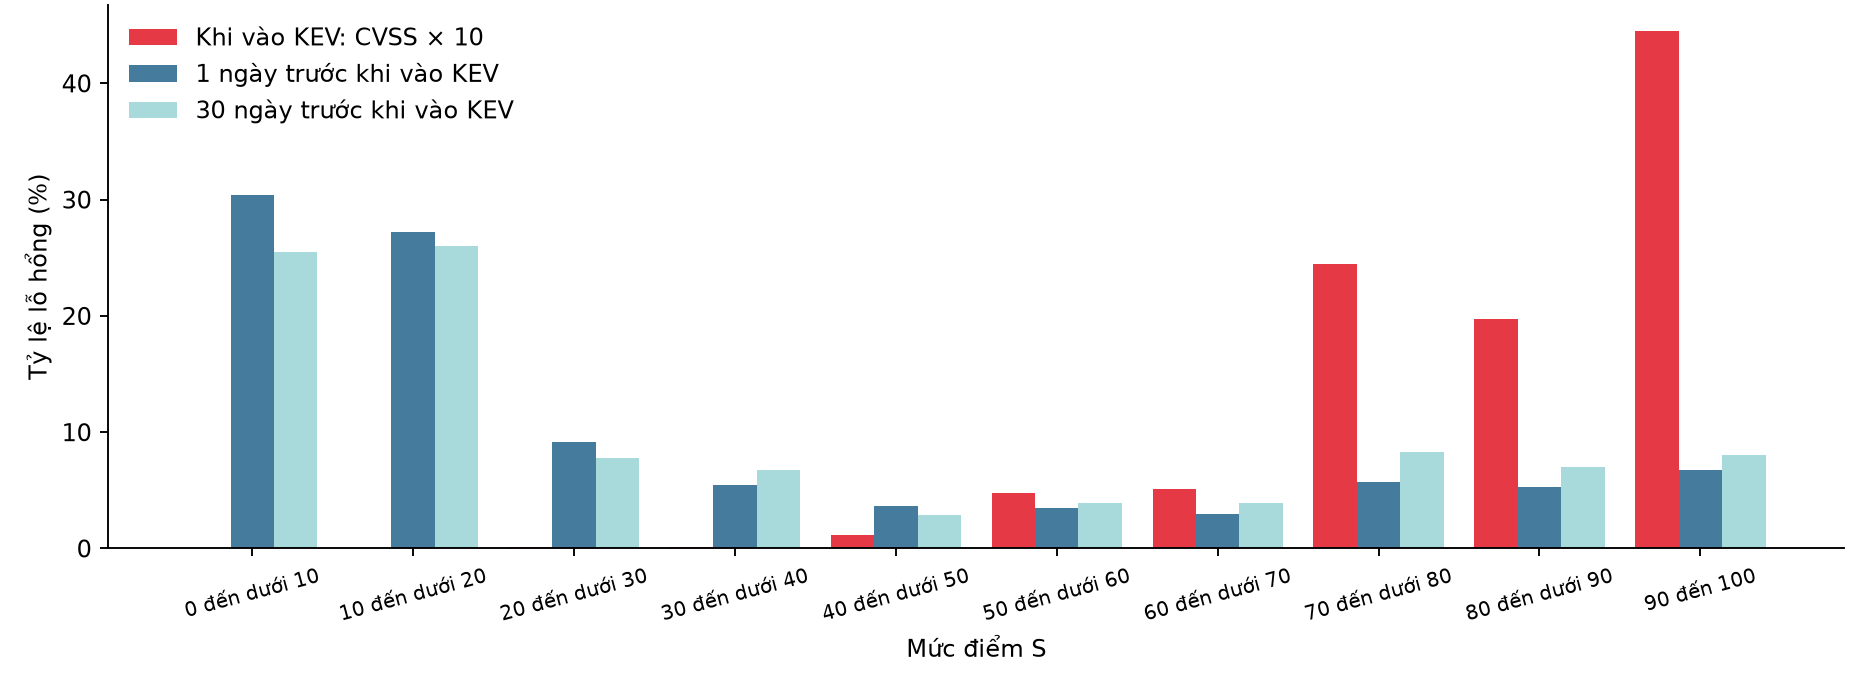
\includegraphics[width=\textwidth]{truoc_kev_muc_diem.png}
\caption{Mức điểm $S$ của 609 lỗ hổng KEV: 30 ngày trước, 1 ngày trước và khi vào KEV.}\label{fig:truockev}
\end{figure}

\begin{table}
\centering
\caption{Trước khi vào KEV, mỗi cách ưu tiên chứa bao nhiêu lỗ hổng sắp vào KEV.}\label{tab:truockev}
\begin{tabular}{lccc}
\toprule
Cách ưu tiên & Chứa được & Khối lượng vá & Gấp ngẫu nhiên \\
\midrule
Quy tắc CSA: CVSS $\ge 8{,}0$ & 64,20\% & 27,73\% & 2,3 \\
$S \ge 30$ (1 ngày trước) & 33,17\% & 8,67\% & 3,8 \\
$S \ge 50$ (1 ngày trước) & 24,14\% & 3,28\% & 7,4 \\
$S \ge 70$ (1 ngày trước) & 17,73\% & 1,34\% & 13,2 \\
\bottomrule
\end{tabular}
\end{table}

\subsection{Kiểm định giả thuyết đặt trước}

\paragraph{H1 -- chưa đạt.} Ở cùng khối lượng vá với quy tắc CSA, gộp 2024 và 2025, công
thức bắt được hơn CVSS 6,0 ca, khoảng tin cậy 95\% $[-2{,}0;\ +15{,}0]$ có chứa 0. Công thức
hơn CVSS ở 2024 (29 so với 27 trên 50) và 2025 (43 so với 39 trên 66), nhưng kém ở 2023 (19,7
so với 24 trên 43). Khi vá ít hơn (phân tích khám phá, không đặt trước), chênh lệch so với
CVSS có ý nghĩa: $+12{,}6$ ca $[+3{,}9;\ +21{,}8]$ khi vá 1\%, $+18{,}2$ ca $[+8{,}3;\ +28{,}5]$
khi vá 5\%. So với EPSS, chênh lệch không có ý nghĩa: $-1{,}0$ $[-3{,}0;\ +2{,}0]$ và $+4{,}4$
$[-0{,}7;\ +10{,}5]$.

\paragraph{H2 -- đạt.} Bảng~\ref{tab:mophong} là kết quả mô phỏng vá hằng tháng với ngân
sách 25\%. Công thức đầy đủ đạt 100\% ``an toàn trong 30 ngày'' ở cả hai năm, trong khi xếp
theo CVSS chỉ đạt 55--56\% và bỏ lại 37--42\% lỗ hổng bị khai thác chưa vá đến cuối kỳ. Cần
lưu ý cây VMC cũng đạt 100\%, và công thức bỏ thành phần KEV chỉ đạt 91--98\%: phần lớn lợi
ích của H2 đến từ \emph{thành phần KEV}, không phải từ cách kết hợp CVSS với EPSS.

\begin{table}
\centering
\caption{Mô phỏng vá hằng tháng, ngân sách 25\% số lỗ hổng trong năm.}\label{tab:mophong}
\begin{tabular}{lcccc}
\toprule
 & \multicolumn{2}{c}{2024 (128 bị khai thác)} & \multicolumn{2}{c}{2025 (172 bị khai thác)} \\
\cmidrule(lr){2-3}\cmidrule(lr){4-5}
Cách chọn & An toàn 30 ngày & Chưa vá & An toàn 30 ngày & Chưa vá \\
\midrule
CVSS                 & 55,5\%  & 42,2\% & 56,4\%  & 37,2\% \\
EPSS                 & 93,8\%  & 3,9\%  & 98,3\%  & 0,6\% \\
Công thức bỏ KEV     & 91,4\%  & 5,5\%  & 98,3\%  & 1,7\% \\
Cây VMC              & 100,0\% & 0,0\%  & 100,0\% & 0,0\% \\
Công thức đầy đủ     & 100,0\% & 0,0\%  & 100,0\% & 0,0\% \\
\bottomrule
\end{tabular}
\end{table}

\paragraph{Lựa chọn số mũ.} Khi chọn số mũ trên dữ liệu năm trước (walk-forward, thử các
giá trị 0,1; 0,2; 0,3; 0,5; 0,7 và 1,0), số mũ được chọn ở cả hai năm kiểm thử là
0,1 chứ không phải 0,3. Trên năm kiểm thử, số mũ 0,1 và 0,3 cho kết quả gần nhau (2025: 43/66
cả hai khi vá bằng khối lượng CSA). Số mũ 0,3 vì vậy là một lựa chọn hợp lý nhưng chưa được
dữ liệu xác nhận là tối ưu.

% =====================================================================
\section{Đánh giá tính khả thi của đề xuất}\label{sec:khathi}
% =====================================================================

\subsection{Khả thi về dữ liệu và kỹ thuật}
\begin{itemize}
\item \textbf{Dữ liệu:} CVSS, EPSS và KEV đều công khai, miễn phí, có API và tệp tải hằng
ngày. EPSS và KEV phủ toàn bộ CVE, không phụ thuộc nhà cung cấp.
\item \textbf{Tính toán:} công thức là một biểu thức đóng, không cần huấn luyện. Chấm điểm
toàn bộ khoảng 210.000 lỗ hổng chỉ là một phép tính vector, mất dưới một giây.
\item \textbf{Tích hợp:} các công cụ quét lỗ hổng đã xuất mã CVE và CVSS; chỉ cần ghép thêm
EPSS và KEV theo mã CVE, cập nhật hằng ngày theo lịch.
\item \textbf{Giải thích được:} khác với mô hình học máy hộp đen, mỗi điểm $S$ tách được thành
ba thừa số rõ nghĩa, phù hợp để đưa vào văn bản chính sách và giải trình với lãnh đạo.
\end{itemize}

\subsection{Khả thi về vận hành}
\begin{itemize}
\item \textbf{Giảm khối lượng vá khẩn cấp.} Thay vì vá khẩn cấp 27,73\% số lỗ hổng như quy
tắc CSA, tổ chức có thể đặt ngưỡng $S \ge 70$ (1,34\%) cho hạn 48 giờ và dùng các ngưỡng
thấp hơn cho hạn dài hơn (ví dụ 7 ngày, 30 ngày).
\item \textbf{Hệ số $AC$ cần dữ liệu nội bộ.} Muốn dùng $AC$, tổ chức phải có danh mục tài
sản phân loại theo mức quan trọng và mức phơi ra Internet. Đây là điều kiện tiên quyết về
quản trị, không phải về kỹ thuật.
\item \textbf{Ngưỡng phải đặt lại định kỳ.} EPSS có nhiều phiên bản mô hình, phân bố điểm
thay đổi theo phiên bản, nên ngưỡng $S$ cần được hiệu chỉnh lại khi FIRST đổi phiên bản.
\end{itemize}

\subsection{Mức độ đã chứng minh}

\begin{table}
\centering
\caption{Tổng hợp mức độ chứng minh của đề xuất.}\label{tab:tonghop}
\begin{tabular}{p{6.6cm}p{4.6cm}}
\toprule
Nhận định & Kết quả \\
\midrule
Ngưỡng CVSS 8,0 vá thừa và bỏ sót nhiều & Đã chứng minh, ổn định qua các năm \\
$S$ cao thì tỷ lệ sắp bị khai thác cao & Đã chứng minh ở 3 ngày đánh giá \\
$S$ tốt hơn CVSS khi vá 1--5\% & Đã chứng minh, gấp 2,7--8,9 lần \\
$S$ tốt hơn CVSS khi vá bằng khối lượng CSA & Chưa ổn định (H1 chưa đạt) \\
Thành phần KEV giúp vá kịp lỗ hổng đã bị khai thác & Đã chứng minh (H2 đạt) \\
$S$ dự báo tốt hơn EPSS dùng riêng & Không chứng minh được \\
Số mũ 0,3 là tối ưu & Không, walk-forward chọn 0,1 \\
Cảnh báo được zero-day & Không thể (27\% lỗ hổng KEV) \\
Hệ số $AC$ cải thiện ưu tiên & Chưa kiểm chứng, thiếu dữ liệu \\
\bottomrule
\end{tabular}
\end{table}

Bảng~\ref{tab:tonghop} tóm tắt mức độ chứng minh. Kết luận về tính khả thi là: công thức
$S$ \emph{khả thi} về dữ liệu, chi phí và vận hành, và \emph{hiệu quả hơn rõ rệt} quy tắc
ngưỡng CVSS khi nguồn lực vá có hạn. Tuy nhiên năng lực dự báo của nó gần như đến hoàn toàn
từ EPSS; thừa số CVSS đóng vai trò đưa mức nghiêm trọng vào thứ tự ưu tiên, không làm dự báo
chính xác hơn.

\subsection{Mối đe dọa đối với tính hợp lệ}
\begin{itemize}
\item \textbf{Căn cứ chưa đầy đủ:} KEV chỉ chứa lỗ hổng CISA xác nhận được, nghiêng về sản
phẩm phổ biến ở Mỹ. Lỗ hổng bị khai thác nhưng chưa vào KEV bị tính là ``không bị khai thác''.
\item \textbf{Số ca dương ít:} mỗi ngày đánh giá chỉ có 61--91 lỗ hổng vào KEV trong 12 tháng,
nên kết quả ở từng mức điểm dao động lớn; chúng tôi dùng bootstrap và lặp ở ba ngày để giảm
ảnh hưởng.
\item \textbf{Thực nghiệm mô tả dùng dữ liệu hiện tại:} Thực nghiệm 1 và bảng phân bổ theo EPSS
dùng trạng thái KEV và EPSS hiện tại, chỉ dùng để mô tả, không dùng để kết luận về dự báo.
\item \textbf{Không có dữ liệu phơi ra Internet:} quy tắc CSA được áp cho mọi lỗ hổng, rộng
hơn phạm vi bài báo đề ra.
\end{itemize}

% =====================================================================
\section{Kết luận}\label{sec:ketluan}
% =====================================================================

Khuyến nghị của CSA vá trong 48 giờ các lỗ hổng CVSS từ 8,0 trên hệ thống phơi ra Internet xuất phát từ một lo ngại có cơ
sở: LLM rút ngắn thời gian từ công bố lỗ hổng tới khai thác. Nhưng dữ liệu cho thấy dùng
CVSS làm tiêu chí duy nhất là không hiệu quả: 98,69\% lỗ hổng trong diện vá khẩn cấp chưa
từng bị khai thác, còn 44,14\% lỗ hổng đã bị khai thác bị bỏ qua. Điều này cũng phù hợp với
chính lời khuyên của bài báo rằng khung ưu tiên phải coi trọng khả năng bị khai thác.

Công thức $S$ kết hợp CVSS, EPSS, KEV và mức quan trọng của tài sản là một thay thế khả thi:
dữ liệu miễn phí, tính toán đơn giản, giải thích được. Khi nguồn lực vá có hạn, nó bắt được
lỗ hổng sắp bị khai thác nhiều gấp vài lần so với xếp theo CVSS, và thành phần KEV bảo đảm
lỗ hổng đã bị khai thác được vá kịp. Về chính sách, chúng tôi khuyến nghị thay ngưỡng CVSS
cố định bằng các mức điểm kết hợp, trong đó lỗ hổng trong KEV và lỗ hổng có EPSS cao trên tài
sản quan trọng được đặt hạn vá ngắn nhất.

Hướng phát triển gồm: kiểm chứng hệ số $AC$ trên dữ liệu tài sản của một tổ chức thực; hiệu
chỉnh số mũ theo từng phiên bản EPSS; và bổ sung tín hiệu sớm hơn EPSS (mã khai thác công
khai, thảo luận trên mạng) để giảm khoảng trễ trước khi lỗ hổng bị khai thác.

\begin{credits}
\subsubsection{\discintname}
Các tác giả không có xung đột lợi ích liên quan tới nội dung báo cáo. Nghiên cứu chỉ dùng dữ
liệu mô tả lỗ hổng công khai; không tạo mã khai thác, không quét hay tấn công hệ thống nào.
\end{credits}

%
% ---- Tai lieu tham khao ----
% Khi chuyen sang BibTeX: \bibliographystyle{splncs04} va \bibliography{tai_lieu}
%
\begin{thebibliography}{99}
\bibitem{csa2026}
Cloud Security Alliance: Automated Exploit Generation: LLMs Cross the Threshold -- From
Vulnerability Discovery to Weaponization. CSA AI Safety Initiative, Unofficial AI-assisted
Research (2026-04-02)

\bibitem{fang2024}
Fang, R., Bindu, R., Gupta, A., Kang, D.: LLM Agents can Autonomously Exploit One-day
Vulnerabilities. arXiv:2404.08144 (2024)

\bibitem{allodi2014}
Allodi, L., Massacci, F.: Comparing Vulnerability Severity and Exploits Using Case-Control
Studies. ACM Transactions on Information and System Security \textbf{17}(1), 1--20 (2014)

\bibitem{jacobs2020}
Jacobs, J., Romanosky, S., Adjerid, I., Baker, W.: Improving Vulnerability Remediation
Through Better Exploit Prediction. Journal of Cybersecurity \textbf{6}(1) (2020)

\bibitem{jacobs2021}
Jacobs, J., Romanosky, S., Edwards, B., Adjerid, I., Roytman, M.: Exploit Prediction Scoring
System (EPSS). Digital Threats: Research and Practice \textbf{2}(3) (2021)

\bibitem{shimizu2026}
% TODO: bo sung tieu de day du cua bai bao
Shimizu, Hashimoto: Cây quyết định VMC kết hợp KEV, EPSS và CVSS để ưu tiên vá lỗ hổng.
IEEE Access (2026)

\bibitem{ssvc}
Spring, J., Hatleback, E., Householder, A., Manion, A., Shick, D.: Prioritizing
Vulnerability Response: A Stakeholder-Specific Vulnerability Categorization. Carnegie Mellon
University, Software Engineering Institute (2019)

\bibitem{cvss31}
FIRST: Common Vulnerability Scoring System v3.1: Specification Document,
\url{https://www.first.org/cvss/v3.1/specification-document}

\bibitem{epss}
FIRST: Exploit Prediction Scoring System (EPSS), \url{https://www.first.org/epss}

\bibitem{nvd}
NIST: National Vulnerability Database, \url{https://nvd.nist.gov}

\bibitem{kev}
CISA: Known Exploited Vulnerabilities Catalog,
\url{https://www.cisa.gov/known-exploited-vulnerabilities-catalog}

\bibitem{bod2201}
CISA: Binding Operational Directive 22-01: Reducing the Significant Risk of Known Exploited
Vulnerabilities (2021), \url{https://www.cisa.gov/binding-operational-directive-22-01}
\end{thebibliography}
\end{document}
